
\index{stones}{$Q_1 \times P_0$ element}
\index{stones}{Penalty Formulation}
\index{stones}{Analytical Solution}

%Taken from aspect manual. 
The SolCx benchmark is intended to test the accuracy of the solution to a problem that has a large jump in the viscosity along a line through the domain. Such situations are common in geophysics: for example, the viscosity in a cold, subducting slab is much larger than in the surrounding, relatively hot mantle material.

The SolCx benchmark computes the Stokes flow field of a fluid driven by spatial density variations, subject to a spatially variable viscosity. Specifically, the domain is $\Omega = [0,1]^2$, gravity is ${\bm g} = (0,-1)^T$ and the density is given by 
\begin{equation}
\rho(x,y) = \sin(\pi y) \cos(\pi x)
\end{equation}
Boundary conditions are free slip on all of the sides of the domain and the temperature plays no role in this benchmark. 
The viscosity is prescribed as follows:
\begin{equation}
\mu(x,y) = 
\left\{
\begin{array}{lll}
1 & for & x<0.5 \\
10^6 & for & x>0.5 \\
\end{array}
\right.
\end{equation}
Note the strongly discontinuous viscosity field yields a stagnant flow 
in the right half of the domain and thereby yields a pressure discontinuity along the interface. 

The SolCx benchmark was previously used in \cite{dumg11} (references to earlier uses of the benchmark are available there) and its analytic solution is given in \cite{zhon96}. It has been carried out in \cite{krhb12} and \cite{gemd13}. 
Note that the source code which evaluates the velocity and pressure fields for both SolCx and SolKz is 
distributed as part of the open source package Underworld (\cite{moql07}, http://underworldproject.org).

In this particular example, the viscosity is computed analytically at the quadrature points (i.e. tracers are 
not used to attribute a viscosity to the element). 
If the number of elements is even in any direction, all elements (and their associated quadrature points)
have a constant viscosity($1$ or  $10^6$). If it is odd, then the elements situated 
at the viscosity jump have half their integration points with $\mu=1$ and half with $\mu=10^6$ 
(which is a pathological case since the used quadrature rule inside elements cannot represent 
accurately such a jump).  


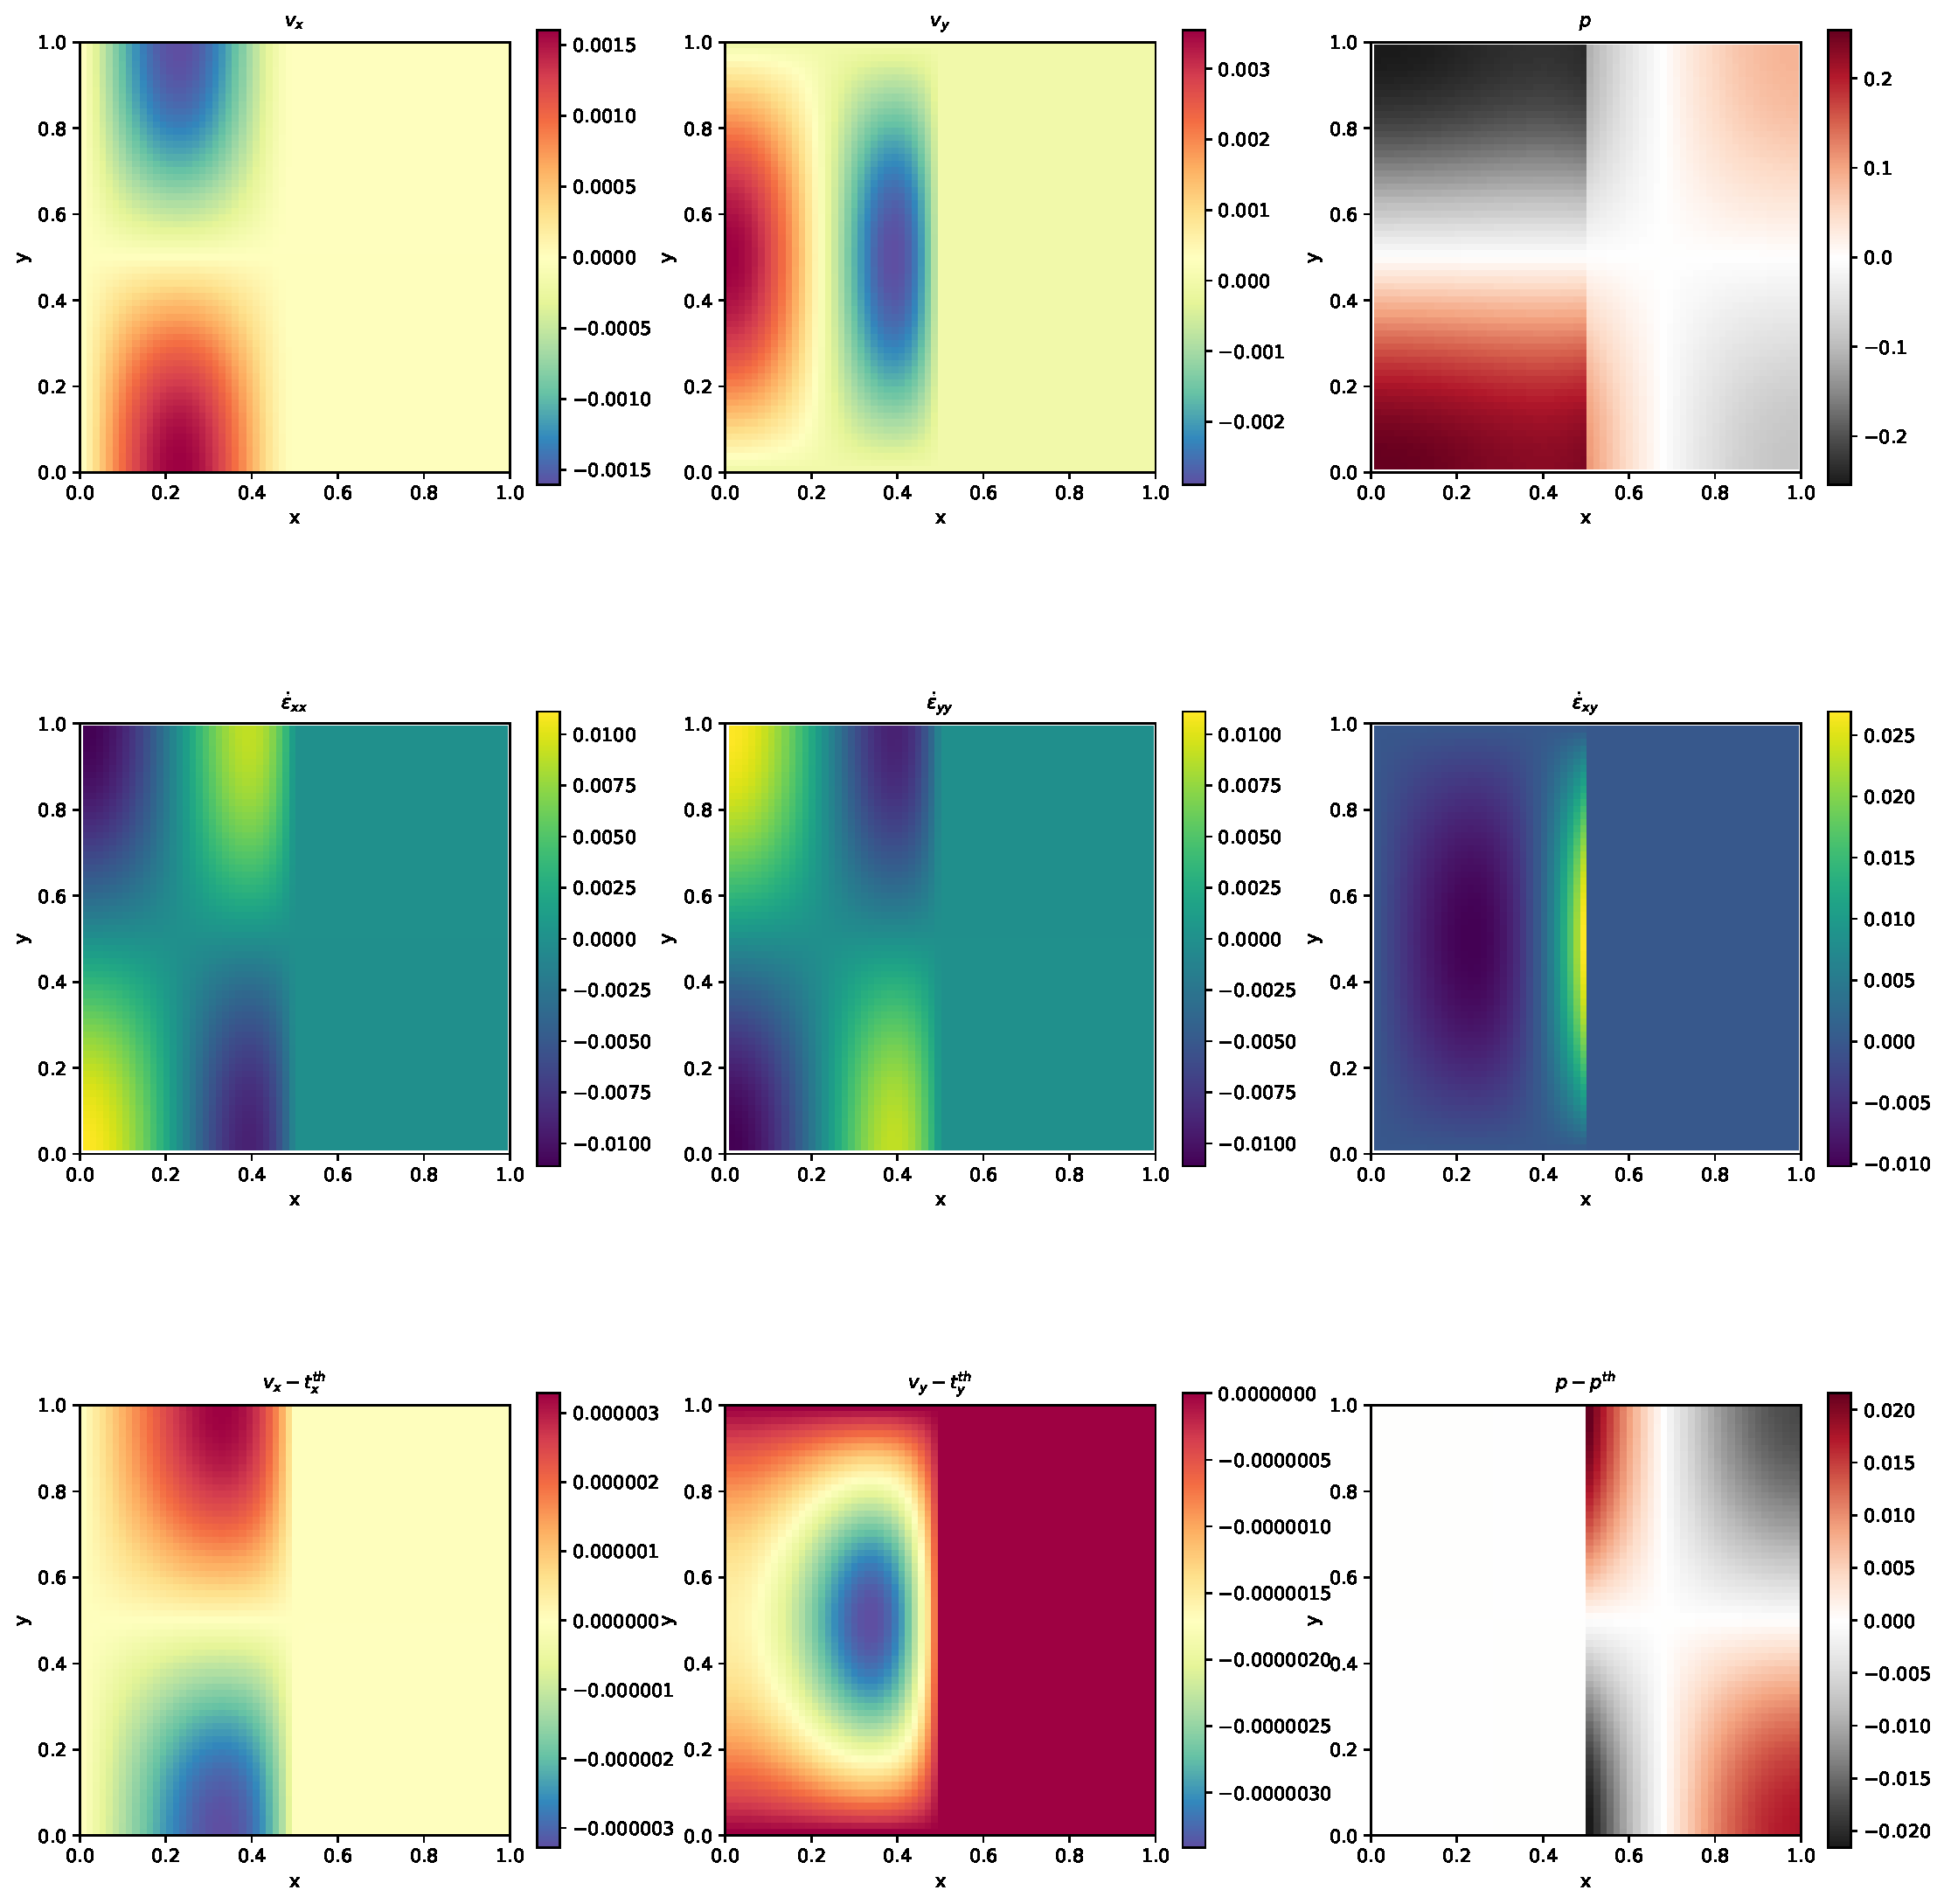
\includegraphics[width=16cm]{python_codes/fieldstone_05/solution.pdf}

\fbox{
\parbox{10cm}{{\bf What we learn from this}
}}



